\documentclass{report}
% \usepackage{darkmode} \enabledarkmode
\usepackage{wrapfig}
%%%%%%%%%%%%%%%%%%%%%%%%%%%%%%%%%
% PACKAGE IMPORTS
%%%%%%%%%%%%%%%%%%%%%%%%%%%%%%%%%


\usepackage[tmargin=2cm,rmargin=1in,lmargin=1in,margin=0.85in,bmargin=2cm,footskip=.2in]{geometry}
\usepackage{amsmath, amsfonts, amsthm, amssymb, mathtools,}
\usepackage[varbb]{newpx}
\usepackage{xfrac}
\usepackage[makeroom]{cancel}
\usepackage{bookmark}
\usepackage{enumitem}
\usepackage{hyperref,theoremref}
\hypersetup{
	pdftitle={Assignment},
	colorlinks=true, linkcolor=overlay!90,
	bookmarksnumbered=true,
	bookmarksopen=true
}
\usepackage[most,many,breakable]{tcolorbox}
\usepackage{xcolor}
\usepackage{varwidth}
\usepackage{varwidth}
\usepackage{etoolbox}
%\usepackage{authblk}
\usepackage{nameref}
\usepackage{multicol,array}
\usepackage{tikz-cd}
\usepackage[ruled,vlined,linesnumbered]{algorithm2e}
\usepackage{comment} % enables the use of multi-line comments (\ifx \fi) 
\usepackage{import}
\usepackage{xifthen}
\usepackage{pdfpages}
\usepackage{transparent}
\usepackage[T1]{fontenc}
\usepackage[utf8]{inputenc}
\usepackage[mathcal]{eucal}
\usepackage{pgfplots}
\pgfplotsset{compat=newest, width=10cm}


\newcommand\mycommfont[1]{\footnotesize\ttfamily\textcolor{iris}{#1}}
\newcommand{\incfig}[1]{%
    \def\svgwidth{\columnwidth}
    \import{../tema_1/figures/}{#1.pdf_tex}
}

\usepackage{tikzsymbols}
\renewcommand\qedsymbol{$\Laughey$}
\usepackage{subcaption}

%\usepackage{import}
%\usepackage{xifthen}
%\usepackage{pdfpages}
%\usepackage{transparent}


%%%%%%%%%%%%%%%%%%%%%%%%%%%%%%
% SELF MADE COLORS
%%%%%%%%%%%%%%%%%%%%%%%%%%%%%%



\definecolor{myg}{RGB}{56, 140, 70}
\definecolor{myb}{RGB}{45, 111, 177}
\definecolor{myr}{RGB}{199, 68, 64}
\definecolor{mytheorembg}{HTML}{F2F2F9}
\definecolor{mytheoremfr}{HTML}{00007B}
\definecolor{mylenmabg}{HTML}{FFFAF8}
\definecolor{mylenmafr}{HTML}{983b0f}
\definecolor{mypropbg}{HTML}{f2fbfc}
\definecolor{mypropfr}{HTML}{191971}
\definecolor{myexamplebg}{HTML}{F2FBF8}
\definecolor{myexamplefr}{HTML}{88D6D1}
\definecolor{myexampleti}{HTML}{2A7F7F}
\definecolor{mydefinitbg}{HTML}{E5E5FF}
\definecolor{mydefinitfr}{HTML}{3F3FA3}
\definecolor{notesgreen}{RGB}{0,162,0}
\definecolor{myp}{RGB}{197, 92, 212}
\definecolor{mygr}{HTML}{2C3338}
\definecolor{myred}{RGB}{127,0,0}
\definecolor{myyellow}{RGB}{169,121,69}
\definecolor{myexercisebg}{HTML}{F2FBF8}
\definecolor{myexercisefg}{HTML}{88D6D1}

%%%%%%%%%%%%%%%%%%%%%%%%%%%%
% Rose Pine 
%%%%%%%%%%%%%%%%%%%%%%%%%%%%
\definecolor{base}{HTML}{191724}
\definecolor{surface}{HTML}{1f1d2e}
\definecolor{overlay}{HTML}{26233a}
\definecolor{muted}{HTML}{6e6a86}
\definecolor{subtle}{HTML}{908caa}
\definecolor{text}{HTML}{e0def4}
\definecolor{love}{HTML}{eb6f92}
\definecolor{gold}{HTML}{f6c177}
\definecolor{rose}{HTML}{ebbcba}
\definecolor{pine}{HTML}{31748f}
\definecolor{foam}{HTML}{9ccfd8}
\definecolor{iris}{HTML}{c4a7e7}


%%%%%%%%%%%%%%%%%%%%%%%%%%%%
% CUSTOM COMMANDS
%%%%%%%%%%%%%%%%%%%%%%%%%%%%

%\fspace{vertical space}
\newcommand{\fspace}[1]{\vspace{#1}\newline}

%\fchapter{chaptercount}{title}
\newcommand{\fchapter}[2]{
  \newpage
  \phantomsection
  \setcounter{chapter}{#1}
\setcounter{section}{0}
\addcontentsline{toc}{chapter}{#2}
}






%%%%%%%%%%%%%%%%%%%%%%%%%%%%
% TCOLORBOX SETUPS
%%%%%%%%%%%%%%%%%%%%%%%%%%%%

\setlength{\parindent}{1cm}
%================================
% THEOREM BOX
%================================

\tcbuselibrary{theorems,skins,hooks}
\newtcbtheorem[number within=section]{Theorem}{Theorem}
{%
	enhanced,
	breakable,
	colback = mytheorembg,
	frame hidden,
	boxrule = 0sp,
	borderline west = {2pt}{0pt}{mytheoremfr},
	sharp corners,
	detach title,
	before upper = \tcbtitle\par\smallskip,
	coltitle = mytheoremfr,
	fonttitle = \bfseries\sffamily,
	description font = \mdseries,
	separator sign none,
	segmentation style={solid, mytheoremfr},
}
{th}

\tcbuselibrary{theorems,skins,hooks}
\newtcbtheorem[number within=chapter]{theorem}{Theorem}
{%
	enhanced,
	breakable,
	colback = mytheorembg,
	frame hidden,
	boxrule = 0sp,
	borderline west = {2pt}{0pt}{mytheoremfr},
	sharp corners,
	detach title,
	before upper = \tcbtitle\par\smallskip,
	coltitle = mytheoremfr,
	fonttitle = \bfseries\sffamily,
	description font = \mdseries,
	separator sign none,
	segmentation style={solid, mytheoremfr},
}
{th}


\tcbuselibrary{theorems,skins,hooks}
\newtcolorbox{Theoremcon}
{%
	enhanced
	,breakable
	,colback = mytheorembg
	,frame hidden
	,boxrule = 0sp
	,borderline west = {2pt}{0pt}{mytheoremfr}
	,sharp corners
	,description font = \mdseries
	,separator sign none
}

%================================
% Corollery
%================================
\tcbuselibrary{theorems,skins,hooks}
\newtcbtheorem[number within=section]{Corollary}{Corollary}
{%
	enhanced
	,breakable
	,colback = iris!25
	,frame hidden
	,boxrule = 0sp
	,borderline west = {2pt}{0pt}{iris!95!black!100}
	,sharp corners
	,detach title
	,before upper = \tcbtitle\par\smallskip
	,coltitle = iris!95!black
	,fonttitle = \bfseries\sffamily
	,description font = \mdseries
	,separator sign none
	,segmentation style={solid, iris!95!black}
}
{th}
\tcbuselibrary{theorems,skins,hooks}
\newtcbtheorem[number within=chapter]{corollary}{Corollary}
{%
	enhanced
	,breakable
	,colback = iris!25
	,frame hidden
	,boxrule = 0sp
	,borderline west = {2pt}{0pt}{iris!95!black}
	,sharp corners
	,detach title
	,before upper = \tcbtitle\par\smallskip
	,coltitle = iris!95!black
	,fonttitle = \bfseries\sffamily
	,description font = \mdseries
	,separator sign none
	,segmentation style={solid, iris!95!black}
}
{th}


%================================
% LENMA
%================================
% this one is in use
\tcbuselibrary{theorems,skins,hooks}
\newtcbtheorem[number within=section]{Lenma}{Lemma}
{%
	enhanced,
	breakable,
	colback = mylenmabg,
	frame hidden,
	boxrule = 0sp,
	borderline west = {2pt}{0pt}{mylenmafr},
	sharp corners,
	detach title,
	before upper = \tcbtitle\par\smallskip,
	coltitle = mylenmafr,
	fonttitle = \bfseries\sffamily,
	description font = \mdseries,
	separator sign none,
	segmentation style={solid, mylenmafr},
}
{th}
% this one is not 
\tcbuselibrary{theorems,skins,hooks}
\newtcbtheorem[number within=chapter]{lenma}{Lemma}
{%
	enhanced,
	breakable,
	colback = mylenmabg,
	frame hidden,
	boxrule = 0sp,
	borderline west = {2pt}{0pt}{mylenmafr},
	sharp corners,
	detach title,
	before upper = \tcbtitle\par\smallskip,
	coltitle = mylenmafr,
	fonttitle = \bfseries\sffamily,
	description font = \mdseries,
	separator sign none,
	segmentation style={solid, mylenmafr},
}
{th}


%================================
% PROPOSITION
%================================

\tcbuselibrary{theorems,skins,hooks}
\newtcbtheorem[number within=section]{Prop}{Proposition}
{%
	enhanced,
	breakable,
	colback = mypropbg,
	frame hidden,
	boxrule = 0sp,
	borderline west = {2pt}{0pt}{mypropfr},
	sharp corners,
	detach title,
	before upper = \tcbtitle\par\smallskip,
	coltitle = mypropfr,
	fonttitle = \bfseries\sffamily,
	description font = \mdseries,
	separator sign none,
	segmentation style={solid, mypropfr},
}
{th}

\tcbuselibrary{theorems,skins,hooks}
\newtcbtheorem[number within=chapter]{prop}{Proposition}
{%
	enhanced,
	breakable,
	colback = mypropbg,
	frame hidden,
	boxrule = 0sp,
	borderline west = {2pt}{0pt}{mypropfr},
	sharp corners,
	detach title,
	before upper = \tcbtitle\par\smallskip,
	coltitle = mypropfr,
	fonttitle = \bfseries\sffamily,
	description font = \mdseries,
	separator sign none,
	segmentation style={solid, mypropfr},
}
{th}


%================================
% CLAIM
%================================

\tcbuselibrary{theorems,skins,hooks}
\newtcbtheorem[number within=section]{claim}{Claim}
{%
	enhanced
	,breakable
	,colback = foam!15
	,frame hidden
	,boxrule = 0sp
	,borderline west = {2pt}{0pt}{foam!100!black}
	,sharp corners
	,detach title
	,before upper = \tcbtitle\par\smallskip
	,coltitle = foam!100!black
	,fonttitle = \bfseries\sffamily
	,description font = \mdseries
	,separator sign none
	,segmentation style={solid, foam!100!black}
}
{th}



%================================
% Exercise
%================================

\tcbuselibrary{theorems,skins,hooks}
\newtcbtheorem[number within=section]{Exercise}{Exercise}
{%
	enhanced,
	breakable,
	colback = myexercisebg,
	frame hidden,
	boxrule = 0sp,
	borderline west = {2pt}{0pt}{myexercisefg},
	sharp corners,
	detach title,
	before upper = \tcbtitle\par\smallskip,
	coltitle = myexercisefg,
	fonttitle = \bfseries\sffamily,
	description font = \mdseries,
	separator sign none,
	segmentation style={solid, myexercisefg},
}
{th}

\tcbuselibrary{theorems,skins,hooks}
\newtcbtheorem[number within=chapter]{exercise}{Exercise}
{%
	enhanced,
	breakable,
	colback = myexercisebg,
	frame hidden,
	boxrule = 0sp,
	borderline west = {2pt}{0pt}{myexercisefg},
	sharp corners,
	detach title,
	before upper = \tcbtitle\par\smallskip,
	coltitle = myexercisefg,
	fonttitle = \bfseries\sffamily,
	description font = \mdseries,
	separator sign none,
	segmentation style={solid, myexercisefg},
}
{th}

%================================
% EXAMPLE BOX
%================================

\newtcbtheorem[number within=section]{Example}{Example}
{%
	colback = myexamplebg
	,breakable
	,colframe = myexamplefr
	,coltitle = myexampleti
	,boxrule = 1pt
	,sharp corners
	,detach title
	,before upper=\tcbtitle\par\smallskip
	,fonttitle = \bfseries
	,description font = \mdseries
	,separator sign none
	,description delimiters parenthesis
}
{ex}

\newtcbtheorem[number within=chapter]{example}{Example}
{%
	colback = myexamplebg
	,breakable
	,colframe = myexamplefr
	,coltitle = myexampleti
	,boxrule = 1pt
	,sharp corners
	,detach title
	,before upper=\tcbtitle\par\smallskip
	,fonttitle = \bfseries
	,description font = \mdseries
	,separator sign none
	,description delimiters parenthesis
}
{ex}

%================================
% DEFINITION BOX
%================================

\newtcbtheorem[number within=section]{Definition}{Definition}{enhanced,
	before skip=2mm,after skip=2mm, colback=gold!10,colframe=love!100,boxrule=0.5mm,
	attach boxed title to top left={xshift=1cm,yshift*=1mm-\tcboxedtitleheight}, varwidth boxed title*=-3cm,
	boxed title style={frame code={
					\path[fill=tcbcolback]
					([yshift=-1mm,xshift=-1mm]frame.north west)
					arc[start angle=0,end angle=180,radius=1mm]
					([yshift=-1mm,xshift=1mm]frame.north east)
					arc[start angle=180,end angle=0,radius=1mm];
					\path[left color=tcbcolback!60!black,right color=tcbcolback!60!black,
						middle color=tcbcolback!80!black]
					([xshift=-2mm]frame.north west) -- ([xshift=2mm]frame.north east)
					[rounded corners=1mm]-- ([xshift=1mm,yshift=-1mm]frame.north east)
					-- (frame.south east) -- (frame.south west)
					-- ([xshift=-1mm,yshift=-1mm]frame.north west)
					[sharp corners]-- cycle;
				},interior engine=empty,
		},
	fonttitle=\bfseries,
	title={#2},#1}{def}
\newtcbtheorem[number within=chapter]{definition}{Definition}{enhanced,
	before skip=2mm,after skip=2mm, colback=gold!10,colframe=rose!100,boxrule=0.5mm,
	attach boxed title to top left={xshift=1cm,yshift*=1mm-\tcboxedtitleheight}, varwidth boxed title*=-3cm,
	boxed title style={frame code={
					\path[fill=tcbcolback]
					([yshift=-1mm,xshift=-1mm]frame.north west)
					arc[start angle=0,end angle=180,radius=1mm]
					([yshift=-1mm,xshift=1mm]frame.north east)
					arc[start angle=180,end angle=0,radius=1mm];
					\path[left color=tcbcolback!60!black,right color=tcbcolback!60!black,
						middle color=tcbcolback!80!black]
					([xshift=-2mm]frame.north west) -- ([xshift=2mm]frame.north east)
					[rounded corners=1mm]-- ([xshift=1mm,yshift=-1mm]frame.north east)
					-- (frame.south east) -- (frame.south west)
					-- ([xshift=-1mm,yshift=-1mm]frame.north west)
					[sharp corners]-- cycle;
				},interior engine=empty,
		},
	fonttitle=\bfseries,
	title={#2},#1}{def}



%================================
% Solution BOX
%================================

\makeatletter
\newtcbtheorem{question}{Question}{enhanced,
	breakable,
	colback=white,
	colframe=gold,
	attach boxed title to top left={yshift*=-\tcboxedtitleheight},
	fonttitle=\bfseries,
	title={#2},
	boxed title size=title,
	boxed title style={%
			sharp corners,
			rounded corners=northwest,
			colback=tcbcolframe,
			boxrule=0pt,
		},
	underlay boxed title={%
			\path[fill=tcbcolframe] (title.south west)--(title.south east)
			to[out=0, in=180] ([xshift=5mm]title.east)--
			(title.center-|frame.east)
			[rounded corners=\kvtcb@arc] |-
			(frame.north) -| cycle;
		},
	#1
}{def}
\makeatother

%================================
% SOLUTION BOX
%================================

\makeatletter
\newtcolorbox{solution}{enhanced,
	breakable,
	colback=white,
	colframe=pine,
	attach boxed title to top left={yshift*=-\tcboxedtitleheight},
	title=Solution,
	boxed title size=title,
	boxed title style={%
			sharp corners,
			rounded corners=northwest,
			colback=tcbcolframe,
			boxrule=0pt,
		},
	underlay boxed title={%
			\path[fill=tcbcolframe] (title.south west)--(title.south east)
			to[out=0, in=180] ([xshift=5mm]title.east)--
			(title.center-|frame.east)
			[rounded corners=\kvtcb@arc] |-
			(frame.north) -| cycle;
		},
}
\makeatother

%================================
% Question BOX
%================================

\makeatletter
\newtcbtheorem{qstion}{Question}{enhanced,
	breakable,
	colback=white,
	colframe=iris,
	attach boxed title to top left={yshift*=-\tcboxedtitleheight},
	fonttitle=\bfseries,
	title={#2},
	boxed title size=title,
	boxed title style={%
			sharp corners,
			rounded corners=northwest,
			colback=tcbcolframe,
			boxrule=0pt,
		},
	underlay boxed title={%
			\path[fill=tcbcolframe] (title.south west)--(title.south east)
			to[out=0, in=180] ([xshift=5mm]title.east)--
			(title.center-|frame.east)
			[rounded corners=\kvtcb@arc] |-
			(frame.north) -| cycle;
		},
	#1
}{def}
\makeatother

\newtcbtheorem[number within=chapter]{wconc}{Wrong Concept}{
	breakable,
	enhanced,
	colback=white,
	colframe=myr,
	arc=0pt,
	outer arc=0pt,
	fonttitle=\bfseries\sffamily\large,
	colbacktitle=myr,
	attach boxed title to top left={},
	boxed title style={
			enhanced,
			skin=enhancedfirst jigsaw,
			arc=3pt,
			bottom=0pt,
			interior style={fill=myr}
		},
	#1
}{def}



%================================
% NOTE BOX
%================================

\usetikzlibrary{arrows,calc,shadows.blur}
\tcbuselibrary{skins}
\newtcolorbox{note}[1][]{%
	enhanced jigsaw,
	colback=rose!10,%
	colframe=iris!90!black,
	size=small,
	boxrule=1pt,
	title=\textbf{Note:},
	halign title=flush center,
	coltitle=white,
	breakable,
	drop shadow=black!50!white,
	attach boxed title to top left={xshift=1cm,yshift=-\tcboxedtitleheight/2,yshifttext=-\tcboxedtitleheight/2},
	minipage boxed title=1.5cm,
	boxed title style={%
			colback=iris!60,
			size=fbox,
			boxrule=1pt,
			boxsep=2pt,
			underlay={%
					\coordinate (dotA) at ($(interior.west) + (-0.5pt,0)$);
					\coordinate (dotB) at ($(interior.east) + (0.5pt,0)$);
					\begin{scope}
						\clip (interior.north west) rectangle ([xshift=3ex]interior.east);
            \filldraw [iris!60, blur shadow={shadow opacity=60, shadow yshift=-.75ex}, rounded corners=2pt] (interior.north west) rectangle (interior.south east);
					\end{scope}
					\begin{scope}[iris!80!black]
						\fill (dotA) circle (2pt);
						\fill (dotB) circle (2pt);
					\end{scope}
				},
		},
	#1,
}

%%%%%%%%%%%%%%%%%%%%%%%%%%%%%%
% SELF MADE COMMANDS
%%%%%%%%%%%%%%%%%%%%%%%%%%%%%%
\newcommand{\boldit}[1]{\begin{bf}\begin{em} #1\end{em}\end{bf}}
\newcommand{\thm}[2]{\begin{Theorem}{#1}{}#2\end{Theorem}}
\newcommand{\cor}[2]{\begin{Corollary}{#1}{}#2\end{Corollary}}
\newcommand{\mlemma}[2]{\begin{Lenma}{#1}{}#2\end{Lenma}}
\newcommand{\mprop}[2]{\begin{Prop}{#1}{}#2\end{Prop}}
\newcommand{\clm}[3]{\begin{claim}{#1}{#2}#3\end{claim}}
\newcommand{\wc}[2]{\begin{wconc}{#1}{}\setlength{\parindent}{1cm}#2\end{wconc}}
\newcommand{\thmcon}[1]{\begin{Theoremcon}{#1}\end{Theoremcon}}
\newcommand{\ex}[2]{\begin{Example}{#1}{}#2\end{Example}}
\newcommand{\dfn}[2]{\begin{Definition}[colbacktitle=love!90!gold]{#1}{}#2\end{Definition}}
\newcommand{\dfnc}[2]{\begin{definition}[colbacktitle=rose!90!gold]{#1}{}#2\end{definition}}
\newcommand{\qs}[2]{\begin{solution}{#1}{}#2\end{solution}}
\newcommand{\pf}[2]{\begin{myproof}[#1]#2\end{myproof}}
\newcommand{\nt}[1]{\begin{note}#1\end{note}}
\newcommand{\commandToText}[1]{\texttt{\string#1}}
\newcommand{\circled}[1]{\tikz[baseline=(char.base)]{
\node[shape=circle,draw,inner sep=1pt] (char) {#1};}}
\newcommand\getcurrentref[1]{%
	\ifnumequal{\value{#1}}{0}
	{??}
	{\the\value{#1}}%
}
\newcommand{\getCurrentSectionNumber}{\getcurrentref{section}}
\newenvironment{myproof}[1][\proofname]{%
	\proof[\bfseries #1: ]%
}{\endproof}

\newcommand{\mclm}[2]{\begin{myclaim}[#1]#2\end{myclaim}}
\newenvironment{myclaim}[1][\claimname]{\proof[\bfseries #1: ]}{}

\newcounter{mylabelcounter}

\makeatletter
\newcommand{\setword}[2]{%
	\phantomsection
	#1\def\@currentlabel{\unexpanded{#1}}\label{#2}%
}
\makeatother




\tikzset{
	symbol/.style={
			draw=none,
			every to/.append style={
					edge node={node [sloped, allow upside down, auto=false]{$#1$}}}
		}
}


% deliminators
\DeclarePairedDelimiter{\abs}{\lvert}{\rvert}
\DeclarePairedDelimiter{\norm}{\lVert}{\rVert}

\DeclarePairedDelimiter{\ceil}{\lceil}{\rceil}
\DeclarePairedDelimiter{\floor}{\lfloor}{\rfloor}
\DeclarePairedDelimiter{\round}{\lfloor}{\rceil}

\newsavebox\diffdbox
\newcommand{\slantedromand}{{\mathpalette\makesl{d}}}
\newcommand{\makesl}[2]{%
\begingroup
\sbox{\diffdbox}{$\mathsurround=0pt#1\mathrm{#2}$}%
\pdfsave
\pdfsetmatrix{1 0 0.2 1}%
\rlap{\usebox{\diffdbox}}%
\pdfrestore
\hskip\wd\diffdbox
\endgroup
}
\newcommand{\dd}[1][]{\ensuremath{\mathop{}\!\ifstrempty{#1}{%
\slantedromand\@ifnextchar^{\hspace{0.2ex}}{\hspace{0.1ex}}}%
{\slantedromand\hspace{0.2ex}^{#1}}}}
\ProvideDocumentCommand\dv{o m g}{%
  \ensuremath{%
    \IfValueTF{#3}{%
      \IfNoValueTF{#1}{%
        \frac{\dd #2}{\dd #3}%
      }{%
        \frac{\dd^{#1} #2}{\dd #3^{#1}}%
      }%
    }{%
      \IfNoValueTF{#1}{%
        \frac{\dd}{\dd #2}%
      }{%
        \frac{\dd^{#1}}{\dd #2^{#1}}%
      }%
    }%
  }%
}
\providecommand*{\pdv}[3][]{\frac{\partial^{#1}#2}{\partial#3^{#1}}}
%  - others
\DeclareMathOperator{\Lap}{\mathcal{L}}
\DeclareMathOperator{\Var}{Var} % varience
\DeclareMathOperator{\Cov}{Cov} % covarience
\DeclareMathOperator{\E}{E} % expected

% Since the amsthm package isn't loaded

% I prefer the slanted \leq
\let\oldleq\leq % save them in case they're every wanted
\let\oldgeq\geq
\renewcommand{\leq}{\leqslant}
\renewcommand{\geq}{\geqslant}

% % redefine matrix env to allow for alignment, use r as default
% \renewcommand*\env@matrix[1][r]{\hskip -\arraycolsep
%     \let\@ifnextchar\new@ifnextchar
%     \array{*\c@MaxMatrixCols #1}}


%\usepackage{framed}
%\usepackage{titletoc}
%\usepackage{etoolbox}
%\usepackage{lmodern}


%\patchcmd{\tableofcontents}{\contentsname}{\sffamily\contentsname}{}{}

%\renewenvironment{leftbar}
%{\def\FrameCommand{\hspace{6em}%
%		{\color{myyellow}\vrule width 2pt depth 6pt}\hspace{1em}}%
%	\MakeFramed{\parshape 1 0cm \dimexpr\textwidth-6em\relax\FrameRestore}\vskip2pt%
%}
%{\endMakeFramed}

%\titlecontents{chapter}
%[0em]{\vspace*{2\baselineskip}}
%{\parbox{4.5em}{%
%		\hfill\Huge\sffamily\bfseries\color{myred}\thecontentspage}%
%	\vspace*{-2.3\baselineskip}\leftbar\textsc{\small\chaptername~\thecontentslabel}\\\sffamily}
%{}{\endleftbar}
%\titlecontents{section}
%[8.4em]
%{\sffamily\contentslabel{3em}}{}{}
%{\hspace{0.5em}\nobreak\itshape\color{myred}\contentspage}
%\titlecontents{subsection}
%[8.4em]
%{\sffamily\contentslabel{3em}}{}{}  
%{\hspace{0.5em}\nobreak\itshape\color{myred}\contentspage}



%%%%%%%%%%%%%%%%%%%%%%%%%%%%%%%%%%%%%%%%%%%
% TABLE OF CONTENTS
%%%%%%%%%%%%%%%%%%%%%%%%%%%%%%%%%%%%%%%%%%%

\usepackage{tikz}
\definecolor{doc}{RGB}{246,193,119}
\usepackage{titletoc}
\usepackage{titlesec}
\contentsmargin{0cm}
\titlelabel{\thetitle. \quad}
\titlecontents{chapter}[3.7pc]
{\addvspace{30pt}%
	\begin{tikzpicture}[remember picture, overlay]%
		\draw[fill=pine!60,draw=pine!60] (-7,-.1) rectangle (-0.9,.5);%
		\pgftext[left,x=-3.5cm,y=0.2cm]{\color{white}\Large\sc\bfseries Chapter\ \thecontentslabel}%
	\end{tikzpicture}\color{pine!60}\large\sc\bfseries}%
{}
{}
{\;\titlerule\;\large\sc\bfseries Page \thecontentspage
	\begin{tikzpicture}[remember picture, overlay]
		\draw[fill=pine!60,draw=pine!60] (2pt,0) rectangle (4,0.1pt);
	\end{tikzpicture}}%
\titlecontents{section}[3.7pc]
{\addvspace{2pt}}
{\contentslabel[\thecontentslabel]{2pc}}
{}
{\hfill\small\bfseries Pg. \thecontentspage}
[]
\titlecontents{subsection}[3.6pc]
{\addvspace{-1pt}\small}
{\qquad\hspace{1.6pc}\contentslabel[\thecontentslabel]{3pc}}
{}
{\hfill\small\bfseries Pg. \thecontentspage}
[]
\makeatletter
\renewcommand{\tableofcontents}{%
	\chapter*{%
	  \vspace*{-20\p@}%
	  \begin{tikzpicture}[remember picture, overlay]%
		  \pgftext[right,x=15cm,y=0.2cm]{\color{pine!60}\Huge\sc\bfseries \contentsname}%
		  \draw[fill=pine!60,draw=pine!60] (13,-.75) rectangle (20,1);%
		  \clip (13,-.75) rectangle (20,1);
		  \pgftext[right,x=15cm,y=0.2cm]{\color{white}\Huge\sc\bfseries \contentsname}%
	  \end{tikzpicture}}%
	\@starttoc{toc}}
\makeatother














%From M275 "Topology" at SJSU
\newcommand{\id}{\mathrm{id}}
\newcommand{\taking}[1]{\xrightarrow{#1}}
\newcommand{\inv}{^{-1}}

%From M170 "Introduction to Graph Theory" at SJSU
\DeclareMathOperator{\diam}{diam}
\DeclareMathOperator{\ord}{ord}
\newcommand{\defeq}{\overset{\mathrm{def}}{=}}

%From the USAMO .tex files
\newcommand{\ts}{\textsuperscript}
\newcommand{\dg}{^\circ}
\newcommand{\ii}{\item}

% % From Math 55 and Math 145 at Harvard
% \newenvironment{subproof}[1][Proof]{%
% \begin{proof}[#1] \renewcommand{\qedsymbol}{$\blacksquare$}}%
% {\end{proof}}

\newcommand{\liff}{\leftrightarrow}
\newcommand{\lthen}{\rightarrow}
\newcommand{\opname}{\operatorname}
\newcommand{\surjto}{\twoheadrightarrow}
\newcommand{\injto}{\hookrightarrow}
\newcommand{\On}{\mathrm{On}} % ordinals
\DeclareMathOperator{\img}{im} % Image
\DeclareMathOperator{\Img}{Im} % Image
\DeclareMathOperator{\coker}{coker} % Cokernel
\DeclareMathOperator{\Coker}{Coker} % Cokernel
\DeclareMathOperator{\Ker}{Ker} % Kernel
\DeclareMathOperator{\rank}{rank}
\DeclareMathOperator{\Spec}{Spec} % spectrum
\DeclareMathOperator{\Tr}{Tr} % trace
\DeclareMathOperator{\pr}{pr} % projection
\DeclareMathOperator{\ext}{ext} % extension
\DeclareMathOperator{\pred}{pred} % predecessor
\DeclareMathOperator{\dom}{dom} % domain
\DeclareMathOperator{\ran}{ran} % range
\DeclareMathOperator{\Hom}{Hom} % homomorphism
\DeclareMathOperator{\Mor}{Mor} % morphisms
\DeclareMathOperator{\End}{End} % endomorphism

\newcommand{\eps}{\epsilon}
\newcommand{\veps}{\varepsilon}
\newcommand{\ol}{\overline}
\newcommand{\ul}{\underline}
\newcommand{\wt}{\widetilde}
\newcommand{\wh}{\widehat}
\newcommand{\vocab}[1]{\textbf{\color{blue} #1}}
\providecommand{\half}{\frac{1}{2}}
\newcommand{\dang}{\measuredangle} %% Directed angle
\newcommand{\ray}[1]{\overrightarrow{#1}}
\newcommand{\seg}[1]{\overline{#1}}
\newcommand{\arc}[1]{\wideparen{#1}}
\DeclareMathOperator{\cis}{cis}
\DeclareMathOperator*{\lcm}{lcm}
\DeclareMathOperator*{\argmin}{arg min}
\DeclareMathOperator*{\argmax}{arg max}
\newcommand{\cycsum}{\sum_{\mathrm{cyc}}}
\newcommand{\symsum}{\sum_{\mathrm{sym}}}
\newcommand{\cycprod}{\prod_{\mathrm{cyc}}}
\newcommand{\symprod}{\prod_{\mathrm{sym}}}
\newcommand{\Qed}{\begin{flushright}\qed\end{flushright}}
\newcommand{\parinn}{\setlength{\parindent}{1cm}}
\newcommand{\parinf}{\setlength{\parindent}{0cm}}
% \newcommand{\norm}{\|\cdot\|}
\newcommand{\inorm}{\norm_{\infty}}
\newcommand{\opensets}{\{V_{\alpha}\}_{\alpha\in I}}
\newcommand{\oset}{V_{\alpha}}
\newcommand{\opset}[1]{V_{\alpha_{#1}}}
\newcommand{\lub}{\text{lub}}
\newcommand{\del}[2]{\frac{\partial #1}{\partial #2}}
\newcommand{\Del}[3]{\frac{\partial^{#1} #2}{\partial^{#1} #3}}
\newcommand{\deld}[2]{\dfrac{\partial #1}{\partial #2}}
\newcommand{\Deld}[3]{\dfrac{\partial^{#1} #2}{\partial^{#1} #3}}
\newcommand{\lm}{\lambda}
\newcommand{\uin}{\mathbin{\rotatebox[origin=c]{90}{$\in$}}}
\newcommand{\usubset}{\mathbin{\rotatebox[origin=c]{90}{$\subset$}}}
\newcommand{\lt}{\left}
\newcommand{\rt}{\right}
\newcommand{\bs}[1]{\boldsymbol{#1}}
\newcommand{\exs}{\exists}
\newcommand{\st}{\strut}
\newcommand{\dps}[1]{\displaystyle{#1}}

\newcommand{\sol}{\setlength{\parindent}{0cm}\textbf{\textit{Solution:}}\setlength{\parindent}{1cm} }
\newcommand{\solve}[1]{\setlength{\parindent}{0cm}\textbf{\textit{Solution: }}\setlength{\parindent}{1cm}#1 \Qed}

% Things Lie
\newcommand{\kb}{\mathfrak b}
\newcommand{\kg}{\mathfrak g}
\newcommand{\kh}{\mathfrak h}
\newcommand{\kn}{\mathfrak n}
\newcommand{\ku}{\mathfrak u}
\newcommand{\kz}{\mathfrak z}
\DeclareMathOperator{\Ext}{Ext} % Ext functor
\DeclareMathOperator{\Tor}{Tor} % Tor functor
\newcommand{\gl}{\opname{\mathfrak{gl}}} % frak gl group
\renewcommand{\sl}{\opname{\mathfrak{sl}}} % frak sl group chktex 6

% More script letters etc.
\newcommand{\SA}{\mathcal A}
\newcommand{\SB}{\mathcal B}
\newcommand{\SC}{\mathcal C}
\newcommand{\SF}{\mathcal F}
\newcommand{\SG}{\mathcal G}
\newcommand{\SH}{\mathcal H}
\newcommand{\OO}{\mathcal O}

\newcommand{\SCA}{\mathscr A}
\newcommand{\SCB}{\mathscr B}
\newcommand{\SCC}{\mathscr C}
\newcommand{\SCD}{\mathscr D}
\newcommand{\SCE}{\mathscr E}
\newcommand{\SCF}{\mathscr F}
\newcommand{\SCG}{\mathscr G}
\newcommand{\SCH}{\mathscr H}

% Mathfrak primes
\newcommand{\km}{\mathfrak m}
\newcommand{\kp}{\mathfrak p}
\newcommand{\kq}{\mathfrak q}

% number sets
\newcommand{\RR}[1][]{\ensuremath{\ifstrempty{#1}{\mathbb{R}}{\mathbb{R}^{#1}}}}
\newcommand{\NN}[1][]{\ensuremath{\ifstrempty{#1}{\mathbb{N}}{\mathbb{N}^{#1}}}}
\newcommand{\ZZ}[1][]{\ensuremath{\ifstrempty{#1}{\mathbb{Z}}{\mathbb{Z}^{#1}}}}
\newcommand{\QQ}[1][]{\ensuremath{\ifstrempty{#1}{\mathbb{Q}}{\mathbb{Q}^{#1}}}}
\newcommand{\CC}[1][]{\ensuremath{\ifstrempty{#1}{\mathbb{C}}{\mathbb{C}^{#1}}}}
\newcommand{\PP}[1][]{\ensuremath{\ifstrempty{#1}{\mathbb{P}}{\mathbb{P}^{#1}}}}
\newcommand{\HH}[1][]{\ensuremath{\ifstrempty{#1}{\mathbb{H}}{\mathbb{H}^{#1}}}}
\newcommand{\FF}[1][]{\ensuremath{\ifstrempty{#1}{\mathbb{F}}{\mathbb{F}^{#1}}}}
% expected value
\newcommand{\EE}{\ensuremath{\mathbb{E}}}
\newcommand{\charin}{\text{ char }}
\DeclareMathOperator{\sign}{sign}
\DeclareMathOperator{\Aut}{Aut}
\DeclareMathOperator{\Inn}{Inn}
\DeclareMathOperator{\Syl}{Syl}
\DeclareMathOperator{\Gal}{Gal}
\DeclareMathOperator{\GL}{GL} % General linear group
\DeclareMathOperator{\SL}{SL} % Special linear group

%---------------------------------------
% BlackBoard Math Fonts :-
%---------------------------------------

%Captital Letters
\newcommand{\bbA}{\mathbb{A}}	\newcommand{\bbB}{\mathbb{B}}
\newcommand{\bbC}{\mathbb{C}}	\newcommand{\bbD}{\mathbb{D}}
\newcommand{\bbE}{\mathbb{E}}	\newcommand{\bbF}{\mathbb{F}}
\newcommand{\bbG}{\mathbb{G}}	\newcommand{\bbH}{\mathbb{H}}
\newcommand{\bbI}{\mathbb{I}}	\newcommand{\bbJ}{\mathbb{J}}
\newcommand{\bbK}{\mathbb{K}}	\newcommand{\bbL}{\mathbb{L}}
\newcommand{\bbM}{\mathbb{M}}	\newcommand{\bbN}{\mathbb{N}}
\newcommand{\bbO}{\mathbb{O}}	\newcommand{\bbP}{\mathbb{P}}
\newcommand{\bbQ}{\mathbb{Q}}	\newcommand{\bbR}{\mathbb{R}}
\newcommand{\bbS}{\mathbb{S}}	\newcommand{\bbT}{\mathbb{T}}
\newcommand{\bbU}{\mathbb{U}}	\newcommand{\bbV}{\mathbb{V}}
\newcommand{\bbW}{\mathbb{W}}	\newcommand{\bbX}{\mathbb{X}}
\newcommand{\bbY}{\mathbb{Y}}	\newcommand{\bbZ}{\mathbb{Z}}

%---------------------------------------
% MathCal Fonts :-
%---------------------------------------

%Captital Letters
\newcommand{\mcA}{\mathcal{A}}	\newcommand{\mcB}{\mathcal{B}}
\newcommand{\mcC}{\mathcal{C}}	\newcommand{\mcD}{\mathcal{D}}
\newcommand{\mcE}{\mathcal{E}}	\newcommand{\mcF}{\mathcal{F}}
\newcommand{\mcG}{\mathcal{G}}	\newcommand{\mcH}{\mathcal{H}}
\newcommand{\mcI}{\mathcal{I}}	\newcommand{\mcJ}{\mathcal{J}}
\newcommand{\mcK}{\mathcal{K}}	\newcommand{\mcL}{\mathcal{L}}
\newcommand{\mcM}{\mathcal{M}}	\newcommand{\mcN}{\mathcal{N}}
\newcommand{\mcO}{\mathcal{O}}	\newcommand{\mcP}{\mathcal{P}}
\newcommand{\mcQ}{\mathcal{Q}}	\newcommand{\mcR}{\mathcal{R}}
\newcommand{\mcS}{\mathcal{S}}	\newcommand{\mcT}{\mathcal{T}}
\newcommand{\mcU}{\mathcal{U}}	\newcommand{\mcV}{\mathcal{V}}
\newcommand{\mcW}{\mathcal{W}}	\newcommand{\mcX}{\mathcal{X}}
\newcommand{\mcY}{\mathcal{Y}}	\newcommand{\mcZ}{\mathcal{Z}}


%---------------------------------------
% Bold Math Fonts :-
%---------------------------------------

%Captital Letters
\newcommand{\bmA}{\boldsymbol{A}}	\newcommand{\bmB}{\boldsymbol{B}}
\newcommand{\bmC}{\boldsymbol{C}}	\newcommand{\bmD}{\boldsymbol{D}}
\newcommand{\bmE}{\boldsymbol{E}}	\newcommand{\bmF}{\boldsymbol{F}}
\newcommand{\bmG}{\boldsymbol{G}}	\newcommand{\bmH}{\boldsymbol{H}}
\newcommand{\bmI}{\boldsymbol{I}}	\newcommand{\bmJ}{\boldsymbol{J}}
\newcommand{\bmK}{\boldsymbol{K}}	\newcommand{\bmL}{\boldsymbol{L}}
\newcommand{\bmM}{\boldsymbol{M}}	\newcommand{\bmN}{\boldsymbol{N}}
\newcommand{\bmO}{\boldsymbol{O}}	\newcommand{\bmP}{\boldsymbol{P}}
\newcommand{\bmQ}{\boldsymbol{Q}}	\newcommand{\bmR}{\boldsymbol{R}}
\newcommand{\bmS}{\boldsymbol{S}}	\newcommand{\bmT}{\boldsymbol{T}}
\newcommand{\bmU}{\boldsymbol{U}}	\newcommand{\bmV}{\boldsymbol{V}}
\newcommand{\bmW}{\boldsymbol{W}}	\newcommand{\bmX}{\boldsymbol{X}}
\newcommand{\bmY}{\boldsymbol{Y}}	\newcommand{\bmZ}{\boldsymbol{Z}}
%Small Letters
\newcommand{\bma}{\boldsymbol{a}}	\newcommand{\bmb}{\boldsymbol{b}}
\newcommand{\bmc}{\boldsymbol{c}}	\newcommand{\bmd}{\boldsymbol{d}}
\newcommand{\bme}{\boldsymbol{e}}	\newcommand{\bmf}{\boldsymbol{f}}
\newcommand{\bmg}{\boldsymbol{g}}	\newcommand{\bmh}{\boldsymbol{h}}
\newcommand{\bmi}{\boldsymbol{i}}	\newcommand{\bmj}{\boldsymbol{j}}
\newcommand{\bmk}{\boldsymbol{k}}	\newcommand{\bml}{\boldsymbol{l}}
\newcommand{\bmm}{\boldsymbol{m}}	\newcommand{\bmn}{\boldsymbol{n}}
\newcommand{\bmo}{\boldsymbol{o}}	\newcommand{\bmp}{\boldsymbol{p}}
\newcommand{\bmq}{\boldsymbol{q}}	\newcommand{\bmr}{\boldsymbol{r}}
\newcommand{\bms}{\boldsymbol{s}}	\newcommand{\bmt}{\boldsymbol{t}}
\newcommand{\bmu}{\boldsymbol{u}}	\newcommand{\bmv}{\boldsymbol{v}}
\newcommand{\bmw}{\boldsymbol{w}}	\newcommand{\bmx}{\boldsymbol{x}}
\newcommand{\bmy}{\boldsymbol{y}}	\newcommand{\bmz}{\boldsymbol{z}}

%---------------------------------------
% Scr Math Fonts :-
%---------------------------------------

\newcommand{\sA}{{\mathscr{A}}}   \newcommand{\sB}{{\mathscr{B}}}
\newcommand{\sC}{{\mathscr{C}}}   \newcommand{\sD}{{\mathscr{D}}}
\newcommand{\sE}{{\mathscr{E}}}   \newcommand{\sF}{{\mathscr{F}}}
\newcommand{\sG}{{\mathscr{G}}}   \newcommand{\sH}{{\mathscr{H}}}
\newcommand{\sI}{{\mathscr{I}}}   \newcommand{\sJ}{{\mathscr{J}}}
\newcommand{\sK}{{\mathscr{K}}}   \newcommand{\sL}{{\mathscr{L}}}
\newcommand{\sM}{{\mathscr{M}}}   \newcommand{\sN}{{\mathscr{N}}}
\newcommand{\sO}{{\mathscr{O}}}   \newcommand{\sP}{{\mathscr{P}}}
\newcommand{\sQ}{{\mathscr{Q}}}   \newcommand{\sR}{{\mathscr{R}}}
\newcommand{\sS}{{\mathscr{S}}}   \newcommand{\sT}{{\mathscr{T}}}
\newcommand{\sU}{{\mathscr{U}}}   \newcommand{\sV}{{\mathscr{V}}}
\newcommand{\sW}{{\mathscr{W}}}   \newcommand{\sX}{{\mathscr{X}}}
\newcommand{\sY}{{\mathscr{Y}}}   \newcommand{\sZ}{{\mathscr{Z}}}


%---------------------------------------
% Math Fraktur Font
%---------------------------------------

%Captital Letters
\newcommand{\mfA}{\mathfrak{A}}	\newcommand{\mfB}{\mathfrak{B}}
\newcommand{\mfC}{\mathfrak{C}}	\newcommand{\mfD}{\mathfrak{D}}
\newcommand{\mfE}{\mathfrak{E}}	\newcommand{\mfF}{\mathfrak{F}}
\newcommand{\mfG}{\mathfrak{G}}	\newcommand{\mfH}{\mathfrak{H}}
\newcommand{\mfI}{\mathfrak{I}}	\newcommand{\mfJ}{\mathfrak{J}}
\newcommand{\mfK}{\mathfrak{K}}	\newcommand{\mfL}{\mathfrak{L}}
\newcommand{\mfM}{\mathfrak{M}}	\newcommand{\mfN}{\mathfrak{N}}
\newcommand{\mfO}{\mathfrak{O}}	\newcommand{\mfP}{\mathfrak{P}}
\newcommand{\mfQ}{\mathfrak{Q}}	\newcommand{\mfR}{\mathfrak{R}}
\newcommand{\mfS}{\mathfrak{S}}	\newcommand{\mfT}{\mathfrak{T}}
\newcommand{\mfU}{\mathfrak{U}}	\newcommand{\mfV}{\mathfrak{V}}
\newcommand{\mfW}{\mathfrak{W}}	\newcommand{\mfX}{\mathfrak{X}}
\newcommand{\mfY}{\mathfrak{Y}}	\newcommand{\mfZ}{\mathfrak{Z}}
%Small Letters
\newcommand{\mfa}{\mathfrak{a}}	\newcommand{\mfb}{\mathfrak{b}}
\newcommand{\mfc}{\mathfrak{c}}	\newcommand{\mfd}{\mathfrak{d}}
\newcommand{\mfe}{\mathfrak{e}}	\newcommand{\mff}{\mathfrak{f}}
\newcommand{\mfg}{\mathfrak{g}}	\newcommand{\mfh}{\mathfrak{h}}
\newcommand{\mfi}{\mathfrak{i}}	\newcommand{\mfj}{\mathfrak{j}}
\newcommand{\mfk}{\mathfrak{k}}	\newcommand{\mfl}{\mathfrak{l}}
\newcommand{\mfm}{\mathfrak{m}}	\newcommand{\mfn}{\mathfrak{n}}
\newcommand{\mfo}{\mathfrak{o}}	\newcommand{\mfp}{\mathfrak{p}}
\newcommand{\mfq}{\mathfrak{q}}	\newcommand{\mfr}{\mathfrak{r}}
\newcommand{\mfs}{\mathfrak{s}}	\newcommand{\mft}{\mathfrak{t}}
\newcommand{\mfu}{\mathfrak{u}}	\newcommand{\mfv}{\mathfrak{v}}
\newcommand{\mfw}{\mathfrak{w}}	\newcommand{\mfx}{\mathfrak{x}}
\newcommand{\mfy}{\mathfrak{y}}	\newcommand{\mfz}{\mathfrak{z}}

\graphicspath{{./figures/}}
\title{\Huge{Maquinas Electricas}}
\author{\large{Daniel Carbajales}}
\date{11 de octubre de 2024}
\hbadness=99999



\begin{document}
 \maketitle
 \newpage
%  |pdfbookmark[<level>]{<tittle>}{<dest>}
 \pdfbookmark[section]{\contentsname}{toc}

 \tableofcontents
 
\fchapter{1}{TEMA 1: Magnetismo y electromagnetismo}\label{chap:1}
  \section{Magnetismo }\label{sec:magnetismo}

 Las maquinas electricas (o maquinas de campo magnético) son un grupo de maquinas que basan su funcionamiento
 en los fenómenos provocados por el magnetismo y el electromagnetismo 
 \dfn{Magnetismo}{Propiedad de algunos materiales en estado natural o para atraer Hierro ("\(\mathbb{Fe}\)")} 
 Los elementos que tienen esta propiedad son denominados \textbf\emph{imanes} son clasficados en:
 \begin{itemize}
   \item\begin{description}
       \item[Imanes permanentes:] Aquellos en los que el efecto de imanación se mantienen de forma continuada.
    \end{description}
  \item\begin{description}
      \item[Imanes temporales:] Aquellos en los que el efecto de imanación se mantiene mientras se produce un efecto de magnetización sobre ellos(\(Ex.\) Electroimanes.)
      \end{description}
 \end{itemize}
 Otra clasificación los divide entre:
 \begin{itemize}
   \item\begin{description}
       \item[Naturales: ] De origen mineral, poseen magnetismo de forma natural. Pueden ser cerámicos o de tierras raras
         \begin{itemize}
           \item\begin{description}
               \item[Cerámicos: ] Formados por bases de oxido de hierro(\(\mathit{Fe_2O_3}\)), estroncio (\(\mathit{SrO}\)) y bario (\(\mathit{BaO}\))   
           \end{description} 
         \item\begin{description}
             \item[Tierras raras: ] Formados por elementos como el neodimio (\(\mathit{Nd}\)) y el samario (\(\mathit{Sm}\)) mucho mas potentes que los 
               imanes cerámicos, con elevada remanencia y resistentes a elevadas temperaturas.  
         \end{description}
         \end{itemize}
    \end{description}
    \item\begin{description}
        \item[Artificiales: ] Su campo magnético es generado mediante un estimulo externo \(\mathit{Ex.}\) holaEl acercamiento de 
        otro{\boldit{imán}} o el paso de una {\boldit{corriente eléctrica}} proxima al metal.
    \end{description}
\end{itemize}
Las partes de los polos con mayor fuerza magnetica se denominan {\boldit{polos}} ({\emph Norte y Sur}) la linea que los une y donde 
hay menor magnetismo se denomina {\boldit{Linea neutra}}.
los principales efectos del magnetismo son la atraccion de los polos {\boldit{"opuestos"}} y la repulsion entre polos {\boldit{"iguales"}}.

\begin{figure}[h]
  \centering
  \caption{Campos magnéticos.}
  \label{fig:magnets}
  \medskip
  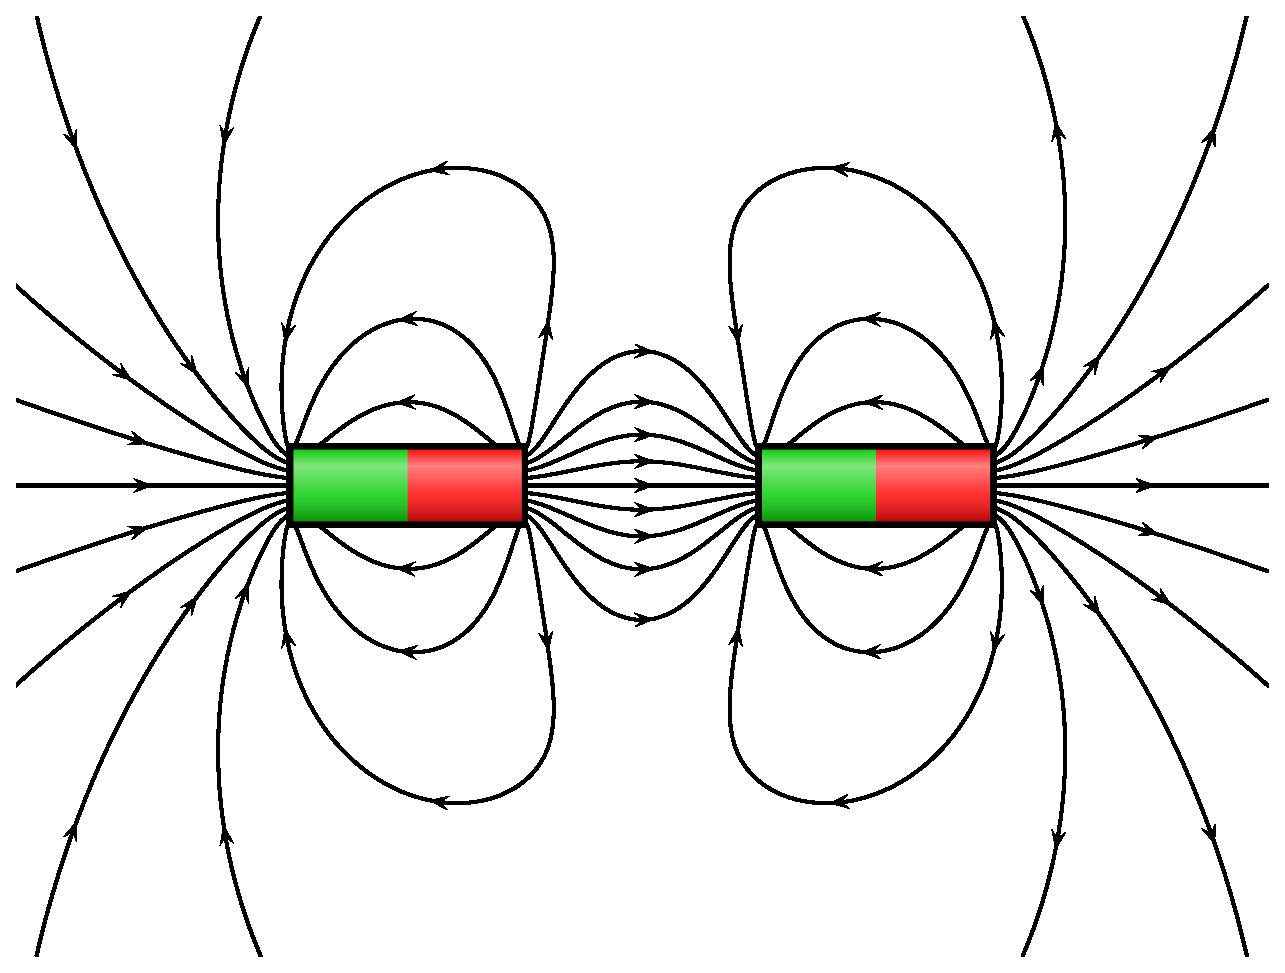
\includegraphics[scale=0.5]{magnets.eps}
\end{figure}

\newpage
  \section{Campo magnético }\label{sec:campo_magnético}
Region del espacio donde se perciben las fuerzas magnéticas de un imán o de un elemento magnetizado  
donde se produce un desplazamiento de cargas de \boldit{norte} a \boldit{sur} representadas graficamente 
las lineas de fuerza\(_{\ref{fig:magnets}}\)
.  Si las lineas de fuerza son de polos opuestos se suman y los imanes se atraen por el 
contrario si las lineas de fuerza son de polos iguales se restan.

  \subsection{Flujo magnético }\label{ssec:Flujo}
№ total de lineas de fuerza que componen un campo magnético. Lo representa "\(\Phi\)" su unidad es el Weber "Wb"

  \subsection{Inducción magnética}\label{ssec:Inducción}
№ de lineas de fuerza que traspasan una unidad de superficie. La {"\boldit{inducción magnética}"} o densidad de flujo magnético 
lo representa la letra \("\beta"\) y su unidad es el Tesla \("T"\)

\begin{center}
  \label{eq:Relacion entre Flujo e Inducción}
  \[\Phi_{(Wb)} = \beta_{\mathit{(T)}} \cdot \mathcal{A}_{(m^2)}\]

Equation: Relacion entre Flujo e Inducción
\end{center}
\nt{El instrumento de medida usado para conocer el valor de inducción magnética de un campo magnético se denomina : {"\boldit{Teslámetro}"}}
\vspace{1em}
  \section{Electromagnetismo }\label{sec:electromagnetismo}

Denominado electromagnetismo, el campo de la electrotecnia que estudia los fenómenos eléctricos y magnéticos
y los efectos que producen.

  \subsection{Campo magnético en un conductor } \label{ssec:campo_magnetico_conductor}
Cuando un conductor recto lo atraviesa una corriente eléctrica se crea un campo magnético cuyas líneas de fuerza son circulares y concentricas al conductor. 
Si queremos conocer el sentido de las lineas de fuerza podemos usar la \boldit{"regla de la mano derecha"} como visto en \ref{fig:Campo Magnetico de un conductor recto}
el pulgar representa \(\mathbf{I}\) y los dedos alrededor del conductor representan \(\mathbf{B}\).
El campo magnético en un coductor recto se encuentra difuminado y no tiene aplicacion practica.
\begin{figure}[h]
  \centering
  \caption{Campo magnetico de un conductor recto.}
  \label{fig:Campo Magnetico de un conductor recto}
  \vspace{.5em}
  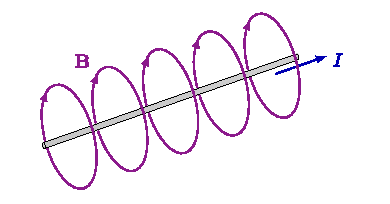
\includegraphics[width=0.45\textwidth]{magnetic_field_wire.pdf}
  \vspace{.5em}
  \begin{center}
    \(\mathbf{B}\): Sentido del campo magnetico  \(\mathbf{I}\): Sentido de la corriente
  \end{center}
\end{figure}
\newpage
  \subsection{Campo magnético en una espira}\label{ssec:espira}
Sin embargo en conductores con forma de espira los campos magnéticos generados tienden a concentrarse en el centro de la espira 
ampliandose la fuerza del campo magnético. Podemos conocer el sentido del campo magnetico en una espira usando el metodo
explicado anteriormente en la \boldit{sección: \ref{ssec:campo_magnetico_conductor}}


  \subsection{Campo magnético en una bobina }\label{ssec:bobina}
En caso de que deseemos conseguir un campo magnético superior al de la espira
podemos unir varias espiras para formar una bobina o "\boldit{solenoide}". {\hspace*{\fill}}
\begin{wrapfigure}[10]{l}{0.55\textwidth}
  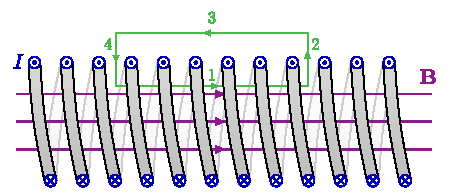
\includegraphics[width=0.5\textwidth]{magnetic_field_solenoid.pdf} 
  \caption{Solenoide}
  \label{fig:solenoide}
\end{wrapfigure}
Usando este metodo podemos sumar los campos magnéticos parciales de las espiras. 
Para conocer el sentido del campo magnetico en una bobina o solenoide podemos usar el metodo explicado en la {\boldit{sección: \ref{ssec:campo_magnetico_conductor}}}
esta vez el sentido de cierre de los dedos alrededor del conductor representa "\(\mathbf{I}\)" (sentido de la corriente) 
y hacia donde apunte el pulgar representa "\(\mathbf{B}\)" (dirección lineas de fuerza).\hfill
\fspace{2em}
\subsection{Intensidad de campo magnético}\label{ssec:intensidad_de_campo_magnético}
Magnitud fisica que indica la fuerza o intensidad del campo magnético. Es representada por la letra \boldit{"\(H\)"}. Su unidad es el amperio-vuelta/metro (\(Av/m \)).\fspace{1em} 
Por lo tanto un campo magnético tiene mayor intensidad cuanto mayor es la corriente "\(I\)" que lo recorre y el № de espiras "\(N\)" que lo forman.
Y sera menor a mayor longitud de la bobina o solenoide \(L\)
\begin{center}
  \label{eq:intensidad_campo_magnetico}
  \begin{math}
    H = \cfrac{N \cdot I}{L}
  \end{math}
  
\end{center}

  \subsection{Fuerza magnetomotriz }\label{ssec:fuerza_magnetomotriz}
Magnitud física que describe la capacidad de un campo magnético de generar flujo magnético entre dos puntos de un circuito electromagnético.
esta magnitud nos permite mantener el campo magnético en un circuito electromagnético. Es representada por la letra \boldit{"\(\mathcal{F}\)"}
y es medida en amperios-vuelta (\( A_v \)). 


\bigskip\begin{flushleft}
Matemáticamente la fuerza magnetomotriz es directamente proporcional a la corriente "\(I\)" del circuito siendo constante 
el número de espiras "\(N\)" que lo forman.
\end{flushleft}
  \begin{center}\[
  \mathcal{F} = N \cdot I
\]\label{eq:fuerza_magnetomotriz}
  \(\mathcal{F}\): Fuerza magnetomotriz \hspace{1.5cm} \(N\): № de espiras \hspace{1.5cm} \(I\): Corriente
  
\end{center}
\vspace{1.5em}
Así podemos afirmar que equ: \ref{eq:intensidad_campo_magnetico} es igual a:
\begin{center}
  \[
    H = \frac{\mathcal{F}}{L}
  \]
\end{center}
\newpage
  \subsection{Circuito magnético }\label{ssec:circuito_magnético}
Si a un solenoide se le introduce una barra ferromagnético en su interior 
los efectos del campo magnético generado aumentan. Por lo que podemos deducir 
que un núcleo de cualquier material ferromagnético dentro de un circuito magnético aumenta la fuerza del campo magnético
sin necesidad de aumentar la corriente \boldit{"\(I\)"}. Las lineas de fuerza dependen de la forma del núcleo ferromagnético
\vspace{1.5em}\newline
El circuito magnético basico es denominado \boldit{"electroimán"} el cual consiste en un nucle ferromagnético y 
una bobina alimentada por una fuente de tensión. Al aplicar una corriente a la bobina, el núcleo es magnetizado
y atrae otros cuerpos ferromagnéticos, sin embargo al cortar la corriente de la bobina el núcleo pierde sus propiedades
magnéticas. 
\vspace{1.5em}\newline
En los circuitos con núcleo magnéticos al calcular la intensidad de campo(\(H\)): \(L\) es el perímetro central del núcleo y no 
la longitud de la bobina.
\vspace{1.5em}
  \subsection{Materiales de los circuitos magnéticos}\label{ssec:materiales_circuitos_magneticos}
Los materiales utilizados en los núcleos de los circuitos magnéticos poseen distintas propiedades
y no todos se comportan igual ante el campo magnético que general o al que se ven expuestos.
En los materiales hay cierto tipo de atomos denominado \boldit{spines} que tienen una orientación magnética propia
y dependiendo de la orientación y magnitud de los spines podemos diferenciar los materiales en:
\begin{itemize}
  
  \item{Diamagnéticos: }
    En estos materiales los spines no tienen campo magnético pero al inducirles un campo magnético sus spines se orientan en el sentido contrario
    del campo magnético inducido. Debido a esta propiedad se dice que los materiales diamagnéticos no interactuan con otros materiales magnéticos.
    \newline(\boldit{\(Ex. \)} Oro, Silicio, Cobre, Hidrógeno, Helio, Germanio, Bronce, Grafito, etc.)
  
  \item{Paramagnéticos: } 
    En estos materiales los spines tienen campo magnético propio y al inducirlos con un campo magnético externo, dichos spines tienden a orientarse
    ligeramente en la direccion del campo magnético.
    \newline(\boldit{\(Ex. \)} Aire, Titanio, Aluminio, etc.)
 
  \item{Ferromagnéticos: }
    En estos materiales los spines tienen campo magnético y al inducirlos con un campo magnético externo, 
    dichos spines tienden a orientarse en la dirección del campo magnético. El hierro es el material por excelencia
    no obstante suele alearse para obtener mejores resultados, como los imanes de \boldit{"neodimio"} (\(Nd_2Fe_{14}B\)).
    \newline(\boldit{\(Ex. \)} Hierro, Cobalto, Níquel, etc.)
\end{itemize}

\begin{figure}[h]%
\centering
\begin{minipage}{.45\textwidth}
      \centering
      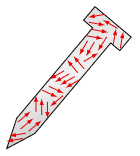
\includegraphics[width=.42\linewidth]{figures/spines_random.pdf}
      \captionof{figure}{Spines en estado natural}
      \label{fig:spines_random}
    
  \end{minipage}%
  \begin{minipage}{.5\textwidth}
    \centering
    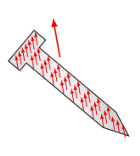
\includegraphics[angle=270, origin=c, width=.45\linewidth]{figures/spines_organized.pdf}
    \captionof{figure}{Spines siguiendo lineas de fuerza}
    \label{fig:spines_organized}
  \end{minipage}
\label{fig:spines}
\end{figure}
\newpage
  \subsection{Reluctancia magnética}\label{ssec:reluctancia}
Al igual que la resistencia "$\Omega$" de un conductor electrico, la Reluctancia "$\mathrm{R}$" es la propiedad que tienen los materiales
ferrmagnéticos de tener una mayor o menor oposición a la formación de líneas de fuerza de un campo magnetico.
\newline\vspace{1em}
Según la \boldit{Ley de Hopkinson}: establecemos la siguiente expresión en la que el flujo magnético "$\Phi$" es directamente proporcional
a la fuerza magnetomotriz "$\mathcal{F}$" e inversamente proporcional a la reluctancia "$\mathrm{R}$":
\begin{figure}[h]
  \[
    \mathrm{\Phi} = \frac{\mathcal{F}}{\mathrm{R}}
  \]
\label{equ:reluctancia}
\end{figure}
\newline Por lo tanto definimos la reluctancia como:
\[
\mathrm{R} = \frac{\mathcal{F}}{\Phi}
\]
\newline Y la fuerza magnetomotriz como:
\[
\mathcal{F} = \Phi \cdot \mathrm{R}
\]

  \subsection{Curva de magnetización}\label{ssec:curva_magnetizada}
Al conectar una fuente de tensión variable a un circuito magnético, y usando un teslámetro para medir la inducción magnética $\beta$ generada
observaremos que en un inicio con poca variación de la intensidad de campo magnético $H$, la $\beta$ aumentara rapidamente
hasta llegar a un punto donde se estabalice, zona la cual es denominada de saturación, debido a que $\beta$ no aumenta aunque $H$ lo haga considerablemente.
\begin{figure}[h]
  \centering
  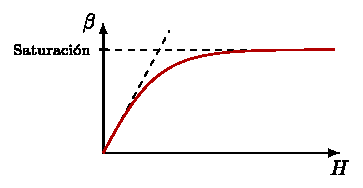
\includegraphics[width=0.65\textwidth]{figures/curva_magnetizacion.pdf}
  \caption{Curva de magnetización}
  \label{fig:curva_magnetizacion}
\end{figure}

\newpage
  \subsection{Permeabilidad magnetica}\label{ssec:permeabilidad_magnetica}
  Es la \boldit{capacidad} que tienen los materiales de magnetizarse, podemos decir que la permeabilidad magnética es la 
  magnitud inversa a la reluctancia. Es representada con la letra \boldit{"\(\mu\)"}(Mu) y su unidad es el \boldit{henrio/metro} ($H/m$). 
  Matemáticamente es la relación entre la inducción "{$\mathbf{\beta}$}" y el campo magnético "{$\mathbf{H}$}"
  \begin{figure}[h]%
    \centering
  \begin{minipage}{.45\textwidth}
    {\LARGE
  $$
  \mu = \frac{\beta}{\mathrm{H}}
$$}
  \label{equ:permeabilidad}
\end{minipage}%
\begin{minipage}{.55\textwidth}
  \centering{
  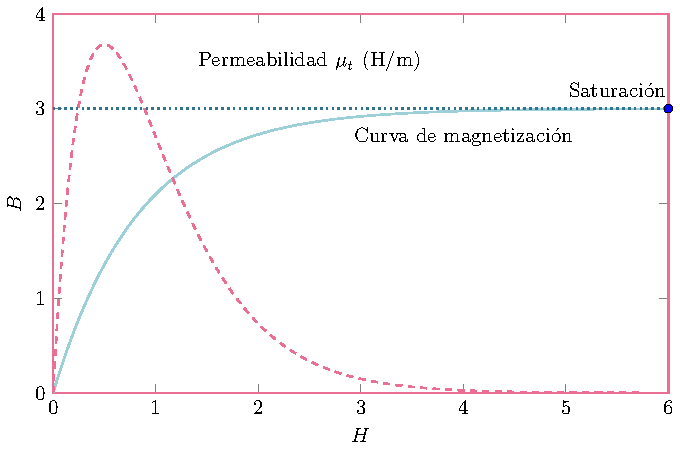
\includegraphics[scale=0.6]{permeability/permeability.pdf}
}
\end{minipage}
\caption{Equ: Permenabilidad magnetica y Curvas}
\end{figure}

  \subsection{Histeresis magnéticaa}\label{ssec:histeresis}
Cuando sometemos a un material ferromagnético a un campo magnético externo, el material presentara
un efecto de \boldit{magnetización}, sin embargo cuando los efectos del campo magnético externo cesan,
podemos observar que los materiales presentan indicios de imanación.
\vspace{1em}\newline
A este efecto se le denomina \boldit{remanencia}, propiedad que tienen los materiales ferromagnéticos 
de mantener los efectos de magnetización una vez finalizado el campo magnético externo.\newline
Aunque la remanencia es favorable en la creación de imanes permanentes es contraproducente para la fabricación de imanes
y máquinas eléctricas; debido a que pueden producir perdidas de enrgía por exceso de calor.
\vspace{1em}
\newline
El estudio de la remanencia se realiza mediante el analisis de lo denominado \boldit{histéresis magnética}. Este proceso
consiste en la representación grafica del comportamiento de un material ferromagnético sometido a un campo magnético del cual
se modifican los valores de $\beta$ y de $\mathrm{H}$ mediante el denominado "\boldit{ciclo de histéresis}".
\begin{figure}[h]
  \vspace{1em}
  \centering 
  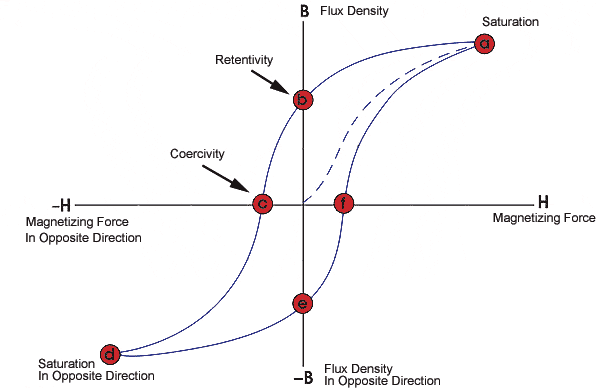
\includegraphics[width=0.65\linewidth]{hysteresis/hysteresis.png}
  \caption{Ciclo de Histéresis}
  \label{fig:hysteresis}

\end{figure}
\newpage
    \subsubsection{Explicación del efecto de histéresis:}
Debemos disponer de un material que no haya sido sometido con anterioridad a un campo magnético:
\begin{enumerate}
  \item Partimos del centro de la grafica y los valores de $\beta$ y $\mathrm{H}$ son van aumentando progresivamente y obtenemos pares de valores
    de ambas magnitudes. Y la curva de imanación progresa como representado la \ref{fig:hysteresis} por la linea 
    discontinua.

  \item Alcanzado el punto de saturacioón (a), los valores de $\beta$ y $\mathrm{H}$ se van disminuyendo con la misma pauta utilizada para 
    la curva anterior. Y observamos que cuando $\mathrm{H}$ es 0, el campo $\beta$ no lo es, presentandose un valor "$\beta_R$" ($R \to$ remanencia).

  \item Si continuamos asignando valores negativos a la intensidad de campo  "$\mathrm{H}$", el campo sera nulo cuando 
    alcanzemos el punto $-H_C$ ($C \to$ coercividad) corespondiente al denominado campo de coercividad. El cual deberemos aplicar a $H$ para que desaparezca
    por completo la remanencia del material.

  \item Si continuamos asignando valores negativos a $\beta$ y $\mathrm{H}$ llegaremos al punto de saturación contrario $m$.

  \item Disminuiremos la asignación de valores a $\beta$ y $\mathrm{H}$ y observaremos que cuando la intensidad de campo $\mathrm{H}$ 
    es 0, el campo $\beta$ no lo es, presentandose un valor "-$\beta_R$" que representa el magnetismo remanante de la polaridad opuesta.
  \item Si continuamos asignando valores positivos a $\mathrm{H}$ y negativos a $\beta$, alcanzaremos el punto $H_C$ contrario
    que necesitaremos aplicar para que el material pierda la remanencia.
\end{enumerate}
\vspace{1.5em}
Podemos clasificar los materiales ferromagnéticos como \boldit{"duros"} y \boldit{"blandos"} en funcion del tamaño de su campo coercitivo.
Usaremos materiales duros para la fabricación de imanes permanentes y materiales blandos para la fabricación de núcleos de máquinas rotativas 
o transformadores.
\fspace{1em}
En la fabricación de máquinas eléctricas deberemos tener en cuenta las pérdidas por histéresis manifestadas en forma de calor,
las cuales son mayores a mayor es el area que abarca la curva del ciclo de histéresis. Por lo que en la fabricación de máquinas eléctricas 
que generen campos variables (como las de corriente alterna) deben fabricarse con los materiales mas blandos posibles.

\vspace{1em}
  \subsection{Corrientes de Foucault}\label{ssec:corrientes_de_foucault}
\begin{wrapfigure}[9]{R}{0.5\textwidth}
  \vspace{-1.5em}
  \centering
  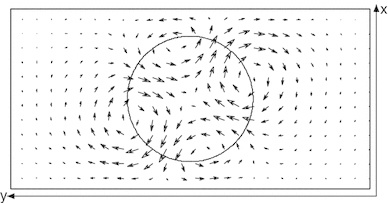
\includegraphics[width=0.5\textwidth]{figures/parasite_currents.png}
  \caption{Corrientes de Foucault}
  \label{fig:parasite_currents}
\end{wrapfigure}
En núcleos ferromagnéticos sometidos a un campo eléctrico se producen unas series de corrientes inducidas 
con forma de bucle en el interior del núcleo, las cuales se oponen a al campo magnético del exterior, 
provocando que los electrones choquen constantemente generando calor y perdidas de energía.
\fspace{1em}
Por este motivo los núcleos de las máquinas eléctricas de corriente alterna se construyen con finas
chapas de hierro al silicio aisladas entre si, lo cual reduce considerablemente las corrientes de Foucault.

\newpage
  \subsection{Fuerza ejercida sobre un conductor por el que circula una corriente}\label{ssec:fuerza_ejercida}
Si se somete a un conductor por el que circula una corriente eléctrica a un campo magnético, el conductor tiende a salir del dicho campo
en el sentido dado por la regla de los tres dedos de la mano izquierda (flemmings left hand rule). La aplicaremos de la siguiente forma:
\begin{itemize}
  \item Dedo índice indica el sentido del campo $\beta$ 
  \item Dedo pulgar indica el sentido de la fuerza $F$
  \item Dedo medio indica el sentido de la corriente eléctrica $I$  
\end{itemize}
\begin{figure}[h]
  \centering
  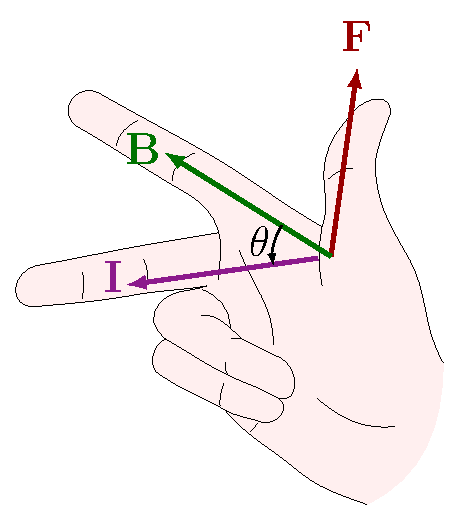
\includegraphics[width=0.25\textwidth]{left-hand/right-hand.pdf}
\end{figure}
\nt{
  También se puede representar el sentido del campo $\beta$ sobre el papel una "$\times$" indicara un campo entrante 
  y un "$\cdot$" indica un campo saliente.
}
\vspace{1.5em}
  \subsection{Fuerza ejercida sobre una espira por la que circula una corriente}\label{ssec:fuerza_espira}


  \subsection{Fuerza electromotriz ejercida en un conductor}\label{ssec:fuerza_electromotriz_conductor}

  \subsection{autoinducción}\label{ssec:autoinducción}


\fchapter{2}{TEMA 2: Materiales y herrramientas del bobinador}\label{chap:2}

  \section{Materiales}\label{sec:materiales}
    \vspace{2em}
    \subsection{Hilo esmaltado}\label{ssec:hilo_esmaltado}
    
      Conductor eléctrico por excelencia utilizado en la fabricacón de circuitos electromagnéticos de maquinas eléctricas.
      Aunque el cobre es el más utilizado en circuitos cuya ligereza sea importante se usara aluminio. Sin embargo el aluminio representa 
      desventajas respecto al cobre, es díficil de soldar sin herramientas especiales y tiene una menor resistencia a las torsiones, lo que facilita
      su rotura y deformcación al manipularlo.
      \fspace{1em}
      Al igual que otros materiales y dispositivos utilizados en electrotecnia, los cables esmaltados estan estandarizados, siendo las principales normas
      las siguientes: 
      \begin{itemize}
        \item{\boldit{IEEC 60317:}}
          Norma de la Comisión Electrotécnica Internacional, usada en Europa y Asia (excepto Japón).
      \item{\boldit{NEMA MW 1000:}}
          Norma de la National Electical Manufacturers Association de Norteamérica, aplicada en Norteamérica y en paises de latinoamérica.
        \item{\boldit{JIS C 3202:}}
          Norma de la Japanese Standards Association y de aplicación exclusiva en Japón.
      \end{itemize}
      \vspace{2em}
      Son comercializados con distintas formas ($Ex.$ Circular, rectangular o cuadrado) distintas geometrías permiten
      aprovechar el espacio de los carretes (transformadores) y los espacios de las ranuras (máquinas rotativas).  
      \fspace{1em}
      Las principales caracteristicas que deberemos conocer son:
      \begin{itemize}
        
        \item{Díametro:} El hilo esmaltado es distribuido por su diametro y no por su sección como los conductores tipicos

        \item{Tipo y espesor del esmalte:} Fabricados usualmente con barnices de poliéster, poliuretano, peliésteramida. Su espesor esta 
          definido por su tensión de ruptura dividendose entre grado 1, grado 2 , grado 3.

        \item{Valor térmico:} Indice maximo para que el conductor trabaje 20.000 horas (a menor temperatura de trabajo 
          mayor es la vida util del conductor).

        \item{Soldabilidad:} Capacidad del conductor para unirse a otros conductores o materiales. expresado en segundos/ temperatura.

        \item{Peso:} El hilo esmaltado a diferencia de los conductores de linea se compra al peso.

        \item{Resistencia eléctrica nominal:} Oposición que presenta el conductor al flujo de corriente elecrtica.

        \item{Tensión de perforación del aislamiento:} Valor en voltios por el que se deteriora el esmalte.

      \end{itemize}
    \vspace{2em}
    \subsection{Carretes para el hilo esmaltado}\label{ssec:carretes_hilo}
      Sirven para empaquetar el hilo esmaltado, al estar normalizados en tamaño y forma permiten su uso en distintas marcas de bobinadoras.
      Son fabricados en distintos tamaños y formas (Cilíndrico, Bicónico y Angular).
    \newpage
    \subsection{Materiales aislantes}\label{ssec:materiales_aislantes}
      Su objetivo es el de aislar los conductores del bobinado, pueden ser sólidos o líquidos, dentro de los sólidos pueden ser,
      rígidos o flexlibles.
      \fspace{1em}
      Al igual que con otros materiales, el fabricante nos proporciona una serie de características las de mayor interés son las siguientes:
      \begin{itemize}

        \item{Espesor:} Dado en milímetros, los materiales de lámina flexible son de 0,1 a 3.00 mm,
          mientrasm que los de tipo rígido pueden tener varios centimetros de grosor

        \item{Rígidez dieléctrica:} Expresado en Kv/mm (Kilovoltios/milímetro) nos da a conocer el limite donde el material pierde
          sus propiedades aislantes.

        \item{Clase térmica:} Temperatura máxima a la que pueden ser sometidos los materiales sin que pierdan sus propiedades 
          aislantes. Normalizado en "Grados celcius" (C).

      \end{itemize}
        \subsubsection{Aislantes flexibles}\label{sssec:aislantes_flexibles}
          Se presentan en láminas de papel o de cartón flexible, utilizados para aislar los devanados una máquina eléctrica
          entre si y con cualquier perte metálica proxima a ellos. Sus principales características son:
          \begin{itemize}
            \item{} Alta resistencia a la abrasión.
            \item{} Buena resistenca termica.
            \item{} Alto poder dieléctrico.
            \item{} bajo indice de absorción de agua y humedad.
          \end{itemize}
          \vspace{1em}
          Uno de los aislantes mas utilizados dentro de esta categoria es el denominado Presspan el cual suele ser combinado con 
          otros materiales ($Ex.$ película de poliéster). No obstante existen otros muchos aislantes que tienen mejores 
          prestaciones tanto mecánicas como eléctricas, que complementas o sustituyen al Presspan. Tales como: 
          El papel crepe, la fibra vulcanizada, el kapton, voltaflex y nomex.

        \subsubsection{Cuñas y aislantes de ranura}\label{sssec:cuñas_y_aislantes_ranura}
          También conocidos como cajetines, son materiales flexibles     

fooking 
hell
/__(...----...)___/
\end{document}
